\chapter{Sina Weibo et le milieu numérique en Chine} 

\newthought{Géant de l'Internet}, la Chine constitue aujourd'hui une des plus grandes figures de l'ordre médiatique mondial. Avec plus de 538 millions d'internautes recensés\footnote{En Juin 2012 d'après  \url{http://www.internetworldstats.com/asia.htm}, consulté le 12 juin 2014 à 14:05}, la présence du Web chinois pèse non seulement dans la balance démographique, mais aussi dans la lecture des fondements politiques du réseau. En effet, le discours et les motivations techno-idéologiques qui ont présidé au développement de l'Internet en Chine diffèrent largement de ces précédents américains et européens. 

Le regard historique que nous allons porter dans la première partie de ce travail rend compte de la lecture des enjeux industriels et politiques qu'ont porté les cadres du Parti Communiste Chinois (PCC) sur les réseaux d'information. La fermeture de \textit{Facebook}, \textit{Youtube} ou \textit{Twitter} relève en effet autant du protectionnisme économique que de la censure médiatique. L'exemple du service de microblog chinois \textit{Sina Weibo}, qui sera l'objet de notre étude, est sans doute un des exemples les plus parlants des bénéfices apportés par le protectionnisme économique aux industries culturelles chinoises. La réussite commerciale de la firme \textit{Sina}, la surveillance constante exercée par le gouvernement et la  possibilité pour les utilisateurs de dialoguer librement sur le service \textit{Weibo} forment un mélange atypique et détonnant que nous allons maintenant décrire.

Tour à tour espace, lieu et territoire, cette plate-forme web articule  différents intérêts et usages dans des dynamiques parfois antagonistes. Cette complexité prend corps dans l'existence géographique de ce réseau en Chine. Une relecture historique de l'évolution du concept de milieu nous amène à proposer le concept très simondonnien de \textit{milieu numérique} pour décrire l’ensemble des protocoles et pratiques discursives qui préside à la création des objets numériques. Nous discuterons également son actualisation sous des forme spécifiques appelées \textit{topogrammes}.


\section{L’Internet chinois : éléments de contexte }
\label{sec:internet-chine}
La production de la recherche en sciences sociales s'est longtemps concentrée autour des intérêts politiques et économiques qui entourent les usages et les modes de diffusion de l’Internet en Chine. Les premières études académiques sont issues du champ de l’information-communication et plus spécifiquement du monde anglo-saxon \citep{Johnson1996,Qiu2005}. Leurs approches reposent sur le postulat qu'Internet serait un outil favorisant la démocratisation. Ainsi cette littérature peut se résumer en un échange d'arguments autour d'une alternative : l'entrée de la Chine dans la ``société de l'information'' va de pair avec la modernisation économique et la démocratisation ou à l’inverse avec un contrôle politique accru de l'information et de la société. Les autorités chinoises craignent en effet de voir se développer de nouveaux canaux de circulation et de nouvelles sources d'information échappant à leur autorité traditionnelle sur les médias - et contestant ainsi leur pouvoir. D'un autre côté, le média internet est également perçu par le gouvernement comme un agent indispensable du processus de modernisation politique et économique (dont l’ouverture de marchés commerciaux intérieurs) permettant de faire circuler l’information de façon optimale, en touchant ainsi l’ensemble des foyers. En somme, un Internet ``sain'' et maîtrisé soutiendrait le développement du système de valeurs gouvernemental, mais également de l’économie et de la culture. Ici, de nombreuses publications se sont également intéressées au rôle de l’économie en ligne dans la croissance économique de la Chine et aux liens étroits des entreprises web avec la censure \citep{Dann2008}. Ces questions de liberté d’expression et du rapport entre démocratie et médias occupent encore aujourd’hui une large place dans la littérature \citep{MacKinnon2009, Douzet2007, Yang2008}.

Les études propres aux usages d’Internet dans le contexte chinois sont toutefois moins nombreuses ou sont généralement le fruit des services marketing des entreprises locales ou internationales en quête de nouveaux marchés \citep{Hwang2005, Bergstrom2012}. Toutefois, on retrouve à la croisée de ces différentes discussions des études plus précises qui cherchent à mettre en relation les dimensions à la fois économique et d’usage du web chinois \citep{Puel2009, Fernandez2010}. Dans le domaine précis de l’analyse des réseaux sociaux - en anglais \textit{Social Network Analysis} (SNA), les publications internationales en sciences sociales concernant la Chine restent encore peu nombreuses. Le champ de la recherche en informatique propose plusieurs études décrivant les dynamiques des échanges de contenus \citep{Yu2011} et les dispositifs de censure en place sur \textit{Sina Weibo} \citep{Bamman2012}. 

Afin de mieux se situer dans le large paysage de cette littérature, cette première partie rend compte des principaux éléments historiques, politiques et économiques d’infra et d’infostructure de l’internet chinois.

\subsection[Petite histoire et évolution de l’Internet chinois]{Petite histoire et évolution de l’Internet chinois}

L’Internet chinois est aujourd’hui le plus grand réseau national, dépassant depuis 2011 l’Amérique du Nord et l’Europe réunies \citep{CNNIC2013}\footnote{538 millions d'utilisateurs alors même que seuls 40\% de ses habitants disposent à ce jour d’une connexion : \textit{`` La collection des données se fait grâce à des logiciels, questionnaires en ligne et sondages par téléphones (…) Pour le CNNIC, un internaute est un citoyen chinois agé de plus de 6 ans qui utilise Internet au moins une heure par semaine ou a utilisé Internet durant les 6 derniers mois ''} (d’après le site officiel de CNNIC, agence officielle du gouvernement).}. Alors que l’installation des infrastructures a débuté seulement en 1996, l’expansion en a été fulgurante \citep{Fang2006}. 51 millions de nouveaux internautes chinois ont fait leur apparition en 2012, soit une hausse de 10\% par rapport à 2011 \citep{CNNIC2013}. 

Comme ailleurs dans le monde, les débuts des réseaux informatiques en Chine se déroulent dans le contexte universitaire avec la création en 1994 du CERNET (\textit{China Education and Research Network}) permettant de relier plusieurs grandes universités du pays. Le 17 mai 1994, la Chine effectue sa première connexion au réseau Internet en se reliant au \textit{Stanford Linear Accelerator Center} (SLAC) de l’Université de Stanford aux États-Unis. L’année suivante, les infrastructures \textit{backbones} nécessaires à l’installation de l’Internet à plus large échelle sont déployées (ChinaNet, GBNet, CERNET) et la première licence d’exploitation commerciale est attribuée, effective dès 1996. Le 1er janvier 1997, le \textit{Quotidien du Peuple} lance sa première version en ligne, devenant alors le premier site Internet d’information officielle du pouvoir central Chinois sur Internet. Dans le courant de l’année, le premier FAI privé chinois \textit{China InfoHighway} voit le jour. En novembre, le CNNIC (\textit{China Internet Network Information Center}) est chargé de recueillir et publier des statistiques sur le développement de l’Internet en Chine \citep{Dai2007}.

Dès son commencement, la mise en place et le contrôle du réseau Internet sont des enjeux importants pour le gouvernement de Pékin. Partie intégrante de leur programme de gouvernance, les dirigeants communistes ont appris depuis longtemps à considérer très sérieusement les nouveaux outils de communication, à la fois comme un risque et une opportunité. Le plus célèbre témoin de cette histoire est sans doute le cinéma soviétique mis en place par Lénine et Trotski dès leur arrivée au pouvoir en 1917. Les \textit{agitki}, courts films de propagande, révèleront de grands cinéastes comme Koulechov, Vertov ou même Eisenstein \citep{Mazuy2002}. Au début des années 90, la Chine s’est engagée depuis plus de 10 ans dans de vastes réformes (\textit{gaige kaifang}) pour se sortir de l’état de chaos où l’avait laissé la Révolution Culturelle. La politique d’ouverture du pays couplée à un fort protectorat ouvre l’ère du \textit{Made in China} qui concerne l’ensemble des secteurs industriels, y compris ceux des médias et télécommunications dont le potentiel stratégique et économique est énorme. Les dirigeants de Pékin sont également bien conscients que la place forte que la Chine réclame dans le paysage mondial se dessinera notamment par une intégration accrue dans le réseau mondial des TIC. Ainsi, en mars 2000 alors que la population des internautes chinois atteint 16,9 millions d’internautes, le premier ministre Jiang Zemin affirme : \textit{“Internet technology is going to change the international situation, military combat, production, culture, and economic aspects of our daily life significantly.”} \citep{Foster2000}

Alors qu’Al Gore et l’administration Clinton déploient les \textit{“information superhighways”} aux États-Unis, le programme d’informatisation et de développement des Technologies de l'Information et de la Communication (TIC) \textit{xinxihua}  devient une des clés du calendrier politique et économique chinois. Jiang Mianheng, le fils du premier ministre Jiang Zemin, est chargé du déploiement de ce vaste projet. Revenu en 1992 après plusieurs années passées dans les universités américaines puis dans la Silicon Valley chez \textit{HP}, Jiang Manheng investit largement dans les infrastructures et soutient dès 1999 le lancement du haut-débit en Chine avec la compagnie \textit{Netcom}, aujourd’hui encore deuxième opérateur du pays \citep{Dai2007}. Fortement influencé par les théories de Alvin Toffler \citep{Tsui2007}, le gouvernement de Jiang Zemin est bien décidé à ne pas rater la \textit{“troisième vague”} de modernisation de l’industrie : l’informatisation. La mise en place d’une quinzaine de \textit{“golden projects”} informe le mouvement de stratégie globale qui doit dynamiser transversalement tous les secteurs d’activité jusqu’au au sein-même de l’administration chinoise. Alors que les \textit{“golden customs”} se chargent des données du commerce extérieur et que la \textit{”golden sea”} devient un outil de communication entre cadres du Parti et administrations locales, les multiples \textit{“golden projects”} sont soutenus par la volonté de mettre en place un \textit{e-government}. Pékin veut faire de l’Internet chinois un espace de dialogue entre citoyens et organes du gouvernement grâce notamment à la mise en place de services administratifs en ligne et d’enquêtes transversales sur la qualité de vie dans les différentes villes de Chine. La gestion proactive de l’Internet national offre également au Parti un vecteur unique pour la diffusion de ses idées politiques. Plusieurs études montrent comment les idées et discours nationalistes sur l’Internet ont bénéficié d’un soutien constant du gouvernement chinois, avec notamment comme objectif l’accès aux communautés chinoises émigrées à l’étranger \citep{Hughes2000}. Finalement, le média Internet doit servir les intérêts du gouvernement et participer à l’unification territoriale, à l’instar des autres médias dits traditionnels comme la télévision.

\subsection[Censure sur l’Internet chinois]{Censure sur l’Internet chinois}
Les modes d’adoption de la technologie Internet par le gouvernement de Pékin illustrent pourtant bien le dilemme constant entre ouverture et protectionnisme qui tiraille la classe politique chinoise depuis la fin de la Révolution Culturelle. L’ouverture au monde et la politique de réformes du \textit{"nouveau départ"} s’accompagnent pour la Chine de nombreux défis souvent considérés comme extérieurs, que résume avec clarté une phrase célèbre attribuée à Deng Xiaoping : \textit{"Lorsque vous ouvrez une fenêtre pour avoir de l’air frais, vous devez vous attendre à ce que quelques mouches rentrent dans la pièce".} Alors que les promesses d’expansion économique et politique de l’Internet sont bien au rendez-vous, les “mouches” entrées par les fenêtres des navigateurs web commencent à essaimer pour faire de plus en plus de bruit.

Depuis 1998, le Ministère de la Sécurité Publique chinois travaille à la conception d’un projet intitulé \textit{Golden Shield} qui constituerait un fichier global des citoyens chinois utilisable tant pour le contrôle de la démographie que le vol de véhicules ou la sécurité aux frontières \citep{Lyons2009}. Lors d’un Trade Show intitulé \textit{"Security China 2000"} se déroulant à Pékin en 2000, le projet est présenté publiquement comme une large base de données devant regrouper les informations administratives des citoyens et leurs activités en ligne dans le but de favoriser le travail de la police \citep{Walton2001}. Titanesque et complexe à réaliser, le projet est peu à peu modifié pour devenir un système de filtrage de contenus et de blocage de sites, basé sur le système du \textit{firewall}. Fang Binxing, un professeur spécialisé dans la sécurité informatique à l’Université de Harbin, est nommé chef-ingénieur du projet \textit{Golden Shield}. Il recrute de nombreux ingénieurs et avec l’aide de l’université de Qinghua et de plusieurs entreprises occidentales (Nortel Networks\footnote{\textit{“Nortel Networks signs contracts valued at over USD 120 Millions during Canadian Prime Minister Jean Chretien’s visit to China”}, PR Newswire, \url{http://www.prnewswire.co.uk/news-releases/nortel-networks-signs-contracts-valued-at-over-us-dollars-120-million-during-canadian-prime-minister-jean-chretiens-visit-to-china-156751255.html}, consulté le 17 février 2014 à 12:18}, Cisco \footnote{\textit{“Cisco Leak: ‘Great Firewall’ of China Was a Chance to Sell More Routers”}, 
Sarah Lai Stirland, 05.20.2008, \url{http://www.wired.com/threatlevel/2008/05/leaked-cisco-do/} consulté le 17 Février 2014 à 12:39}). Ensemble, ils s’attèlent au développement technologique du projet qui devait devenir le système de contrôle de l’Internet chinois aujourd’hui en activité. Baptisé de manière informelle \textit{“The Great Firewall”} (GFW) par analogie avec la \textit{"Grande Muraille de Chine”} (Great Wall), ce système `` sociotechnique '' hors du commun est aujourd’hui considéré comme une des plus grandes installations d’analyse et de traitement de données en activité. À chaque seconde, GFW traite et scanne des millions de chaines de caractères issues des requêtes et pages vues par des centaines de millions d’internautes \citep{Winter2012}. Au-delà de la censure automatique, GFW emploierait aujourd’hui entre 30 000 et 50 000 personnes\footnote{\textit{"What is internet censorship?"}. Amnesty International Australia. 28 Mars 2008. Consulté le 17 Février 2014 à 15h12} : ingénieurs, modérateurs, relecteurs, officiers de police, etc. Phénomène particulier, un groupe de rédacteurs est notamment chargé d’intervenir dans les discussions ou les forums en ligne pour faire valoir le point de vue officiel. L’adage veut que chacun des messages posté soit rémunéré 50 centimes RMB, ce qui a amené les internautes chinois à baptiser non sans humour ces représentants de l’ordre politique en ligne \textit{“le Parti à 50 centimes” (wumao dang)}.

\begin{figure}[htbp]
    \centering
    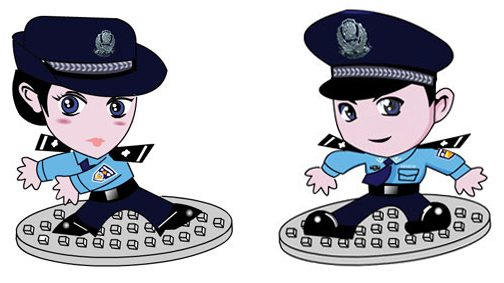
\includegraphics{figures/chap1/jingcha.jpg}
    \caption[Jingjing et Chacha, les policiers de l'Internet chinois]{\textit{Jingjing} et \textit{Chacha} sont deux figures créées par les autorités chinoises pour signifier la présence policière en ligne aux internautes. Le nom de ces veilleurs dessinés est une composition issue du mot “police” en chinois (\textit{jingcha}). Source : \url{http://jswm.newssc.org/system/2008/10/29/011233423.shtml} consultée le 17 Février 2014, à 15:32}
    \label{fig:jingcha}
\end{figure}

Au-delà de l’activité manuelle de milliers d’employés, GFW opère également plusieurs types de blocages sur les contenus. Techniquement, la plupart des filtrages se déroulent au niveau du fournisseur d’accès avec notamment des adresses particulières qui sont rendues inaccessibles : l’adresse \textit{facebook.com} ou \textit{youtube.com} renvoie une erreur “404 : Le site demandé n’existe pas”. Ainsi, de nombreux sites célèbres ne sont pas accessibles (\textit{Twitter}, \textit{Youtube}, \textit{Facebook}, etc.) Les autres blocages effectifs s’effectuent selon les adresses IP ou les serveurs d’attribution de noms de domaine (DNS) menant parfois au blocage de serveurs entiers \citep{Winter2012}. Les URLs des pages de certains sites importants sont également filtrées. Sur Wikipedia notamment, la page \textit{“Tiananmen Square protests of 1989”} est inaccessible depuis la Chine sans que le site Wikipedia soit pour autant intégralement bloqué. Également, des requêtes contenant des mots “interdits” sur les moteurs de recherche peuvent conduire à des micro-coupures ou un accès restreint au web pendant parfois plusieurs minutes\footnote{Testé depuis Shanghai en Septembre 2013.}. La liste des sites et mots bloqués n’est pas publiée par le gouvernement et l’ajout sur ses listes s’effectue a priori sur la demande de différentes agences gouvernementales chinoises, sans notification publique. Essentiellement, il s’agit de sites à caractère pornographique (la pornographie est illégale en Chine), de sites liés aux groupes dissidents chinois (Falung Gong, Dalai Lama, Tibet Libre...), de sites du gouvernement taiwanais et d’autres sites revendiquant la liberté d’expression pour la Chine\footnote{Si ces sites ne sont pas publiés officiellement, une liste est néanmoins maintenue par une entreprise privée sur le site http://www.greatfirewall.biz, consulté le 17 février 2014.}.

Si le GFW est un outil de contrôle politique, il participe également largement au protectorat économique chinois. L’expansion rapide du vaste marché de l'Internet en Chine s’est faite sous un strict contrôle politique et si l’État a largement financé les infrastructures, GFW a été l’un des moteurs de la croissance des grandes sociétés du web chinois. L'absence du géant \textit{YouTube} a notamment permis aux acteurs locaux de la vidéo en ligne de se développer rapidement. \textit{Youku}, son homogue chinois, est aujourd’hui sujet à une valorisation colossale sur les marchés d’affaires. La situation est similaire pour les réseaux sociaux. L'absence de concurrence étrangère due à l’interdiction de \textit{Facebook} en 2008 puis \textit{Twitter} en 2009 a permis aux acteurs chinois de se développer. Leur poids sur le marché intérieur les autorise aujourd’hui à rivaliser avec leurs concurrents américains au niveau mondial tant en nombre d’utilisateurs qu’en revenus directs et indirects générés \citep{CIW2012}.

Ainsi, GFW a affecté l’économie du pays en profondeur et à ce titre notamment continue d’être une préoccupation première du pouvoir politique. L’évolution technologique de GFW suit de près l’évolution des moyens de contournement des blocages, qui sont nombreux. Le célèbre logiciel \textit{Tor} garantissant l’anonymat sur Internet est aujourd’hui bloqué en Chine \citep{Winter2012} ainsi que d’autres technologies communes d’anonymisation (comme le proxy notamment). Pourtant, il reste très facile de \textit{``faire le mur''(fanqiang)} et d’accéder aux contenus en contournant les limites du GFW. Les solutions techniques à disposition sont multiples et souvent peu coûteuses à mettre en place ou à utiliser. De nombreux services commerciaux proposent de se connecter depuis d’autres pays à l’aide d’un VPN (\textit{Virtual Private Network}) pour un coût très faible. Le VPN permet d'accéder au Web depuis une machine située dans un autre pays et de bénéficier ainsi de l’accès tel qu’il existe dans le pays où se situe la machine. Le flou juridique qui entoure l’existence de services commerciaux de contournement de GFW témoigne de l’intérêt du gouvernement chinois à protéger largement le marché intérieur en supprimant l’accès aux services majoritaires du web occidental, sans pour autant exercer une traque systématique de chaque personne voulant utiliser \textit{Facebook} ou \textit{Gmail}. De plus, l’absence totale de moyens de contournement interdirait l’accès à des sources précieuses d’informations professionnelles (notamment \textit{Twitter}). Les autorités chinoises ne semblent pas prêt à payer le prix de cette perte d’avantages concurrentiels décisifs pour les entreprises chinoises. Une étude de l’OpenITP parue en 2013 analyse l’usage des outils de contournement de la censure auprès d’un échantillon de 1175 utilisateurs en Chine. Au-delà des solutions technologiques variées, on peut noter que la première raison pour contourner le blocage de l’Internet est l’utilisation des services de \textit{Google} (notamment de \textit{Gmail})\footnote{Bloqué en Chine, testé en Juin 2014 à Shanghai et Shenzhen}, suivi de la volonté de se rendre sur les sites de réseaux sociaux américains comme \textit{Facebook} et \textit{Twitter}, puis de l’accès aux contenus d’actualité, de vidéo en ligne et de sites à caractère pornographique. Les utilisateurs souhaitant accéder à des contenus à caractère politique ou utilisant l’Internet de manière anonyme pour communiquer de façon plus sécurisée représentent moins de 10\% de la population étudiée \citep{OpenITP2013}. Il est également important de noter que l’immense majorité des internautes chinois n’utilise pas de système de contournement des blocages de l’Internet. 

\section[Médias sociaux en Chine : un paysage morcelé]{Médias sociaux en Chine : un paysage morcelé}

Alors qu’un blocage officiel s’applique sur les plus célèbres sites Internet californiens, de nombreux services se sont développés pour répondre aux besoins et intérêts des internautes chinois. Cette culture particulière des entreprises politiques et économiques du web chinois influe sur l’être-ensemble des usagers et les contenus diffusés sur le réseau.

Profitant de l’absence des grands noms du réseau social en ligne, de nombreux services ont vu le jour sur la Toile chinoise. L'importance du \textit{guanxi} \citep{Yu2008}, élément profond de la culture traditionnelle poussant chaque Chinois à entretenir et exposer avec soin ses relations en société, peut également avoir contribué à créer un terrain idéal pour le développement rapide de ces sites \citep{Yang2011b}. Plutôt morcelé, le paysage des SNS en Chine offre une variété de services et d’acteurs qui rassemble les internautes chinois selon leurs centres d'intérêts. \textit{Douban} offre aux jeunes ``branchés'' de partager lectures, films et musique. \textit{Kaixin001}, plus centré sur les jeux, propose un espace ludique pour les trentenaires au bureau. \textit{Renren} (anciennement \textit{Xiaonei}) est, quant à lui, un véritable clone de \textit{Facebook} et se focalise sur le monde étudiant chinois \citep{Renaud2011}. Malgré ces nombreux concurrents, le service de messagerie instantanée \textit{QQ} reste le leader incontesté du marché chinois. Aujourd’hui classé 8ème site le plus visité au monde\footnote{D’après Alexa.com, consulté le 3 Février 2013.}, \textit{QQ} dénombre jusqu’à 100 millions d’utilisateurs connectés simultanément\footnote{Voir \url{http://im.qq.com/culture}, consulté le 14 Février 2013.}. Quatrième plus grande firme du web mondial, son créateur le géant \textit{Tencent Holdings Limited} a investi depuis le début de l’Internet en Chine dans de nombreux domaines des TIC : jeux, publicité en ligne, e-commerce, etc. Plus qu’une simple messagerie de chat, les services de \textit{QQ} sont multiples : la page de profil de chaque utilisateur (\textit{QZone}) permet de maintenir un blog et d’écouter de la musique (\textit{QQmusic}). Chaque utilisateur peut se créer un avatar en ligne pouvant revêtir de nombreux vêtements et accessoires vendus en ligne (\textit{QQshow}) mais aussi participer à de nombreux jeux multi-joueurs pour tous les âges (\textit{QQ Entertainement}). Le système de monnaie virtuelle (\textit{QCoin}) mis en place pour les achats en ligne a généré dès son lancement en 2005 un nombre important de transactions\footnote{\textit{Central Bank alert on ``virtual money''}, People’s Daily, 12 Janvier 2007, \url{http://english.people.com.cn/200701/12/eng20070112_340681.html} consulté le 28 Mai 2014}, poussant même \textit{Tencent} à obtenir une licence bancaire. L’utilisation de la messagerie \textit{QQ}, réseau social avant l’heure, est devenue un véritable phénomène de société porté par la diversification de \textit{Tencent} dans de multiples secteurs sous une marque unique. Au-delà des jeunes et des professionnels de l’Internet, le réseau \textit{QQ} comptait en juillet 2011 plus de 812,3 millions de comptes actifs, faisant de lui le deuxième réseau social mondial après \textit{Facebook}. Du magasin de photocopie de quartier au réseau de prostitution clandestin, \textit{QQ} héberge les discussions quotidiennes et fait pour ainsi dire partie intégrante du paysage des villes modernes. Les chinois échangent plus volontiers leurs numéros de \textit{QQ} que ceux de leurs téléphones portables et ce mode de communication est souvent préféré au mail dans les échanges au bureau. Convergeant rapidement avec la croissance fulgurante du e-commerce en Chine, les produits dérivés estampillés \textit{QQ} sont devenus une véritable mode en Chine : voitures, téléphones, boissons, etc. Le groupe \textit{Tencent} poursuit son évolution avec le lancement en 2008 de son service de microblog \textit{Tencent Weibo}, qui a connu un véritable succès dès les premiers mois. Aujourd’hui, la firme de Shenzhen continue la conversion de ces utilisateurs \textit{QQ} vers sa plate-forme mobile \textit{WeChat} qui connaît actuellement une très forte croissance, au point de voir les autres services de microblog mis au banc par les utilisateurs. Messagerie écrite et vocale, \textit{WeChat} se diversifie en offrant désormais d’utiliser son compte \textit{QQ} comme moyen de paiement pour de nombreux services du quotidien (taxis, nourritures, etc.)\footnote{\textit{21 million taxi rides have been booked on WeChat in the past month}, Tech in Asia February 12, 2014 \url{http://www.techinasia.com/wechat-21-million-taxi-rides-booked} consulté le 17 Février 2014 à 15:36}.

\subsection[Microblog en Chine et Sina Weibo]{Microblog en Chine et Sina Weibo}
Les sites de \textit{microblogging} (en chinois \textit{weibo}) permettent aux utilisateurs de poster de courts messages composés de photos ou de texte de 140 caractères maximum, puis de les commenter et de les partager avec leurs lecteurs. A l’image de \textit{Twitter}, chaque utilisateur peut souscrire aux fils d’info d’autres utilisateurs afin de recevoir leurs messages et mises à jour.

L’histoire du microblog en Chine débute en 2007 avec plusieurs services se présentant alors comme des clones de \textit{Twitter}. Le service \textit{Fanfou} connaît notamment un succès rapide. De nombreux journalistes l’utilisent pour enquêter et coordonner leurs actions lors de l’arrivée du SRAS ou le tremblement de terre de Wenchuan dans le Sichuan en 2008. \textit{Fanfou} est fermé sur ordre du gouvernement en juillet 2009, suite aux nombreux commentaires suscités par des émeutes s’étant déroulées à Urumqi dans la province du Xinjiang. A peine un mois après cette fermeture, la firme \textit{SINA Corporation} saisit l’opportunité et s’installe en lançant son propre service de microblog intitulé \textit{Sina Weibo}. \textit{Sina Weibo} connaît dès son lancement une croissante soutenue avec plus de 10 millions de nouveaux inscrits par mois et devient en 2012 la plateforme de microblog la plus utilisée en Chine avec 250 millions d’utilisateurs \citep{McKinsey2012}. Les revenus de \textit{Sina Weibo} ne cessent alors de croître (+19\% en 2012\footnote{Voir \url{http://corp.sina.com.cn/chn/Annual_Report_2011_Final.pdf}, consulté le 16/02/2013.}) alors que plus de 86 millions de messages sont postés chaque jour sur ce service\footnote{D’après Sina Corp. Earning Calls - \url{http://phx.corporate-ir.net/phoenix.zhtml?c=121288&p=irol-EventDetails&EventId=4727394}, consulté le 16/02/2013}. 


\begin{figure}[htbp]
    \centering
    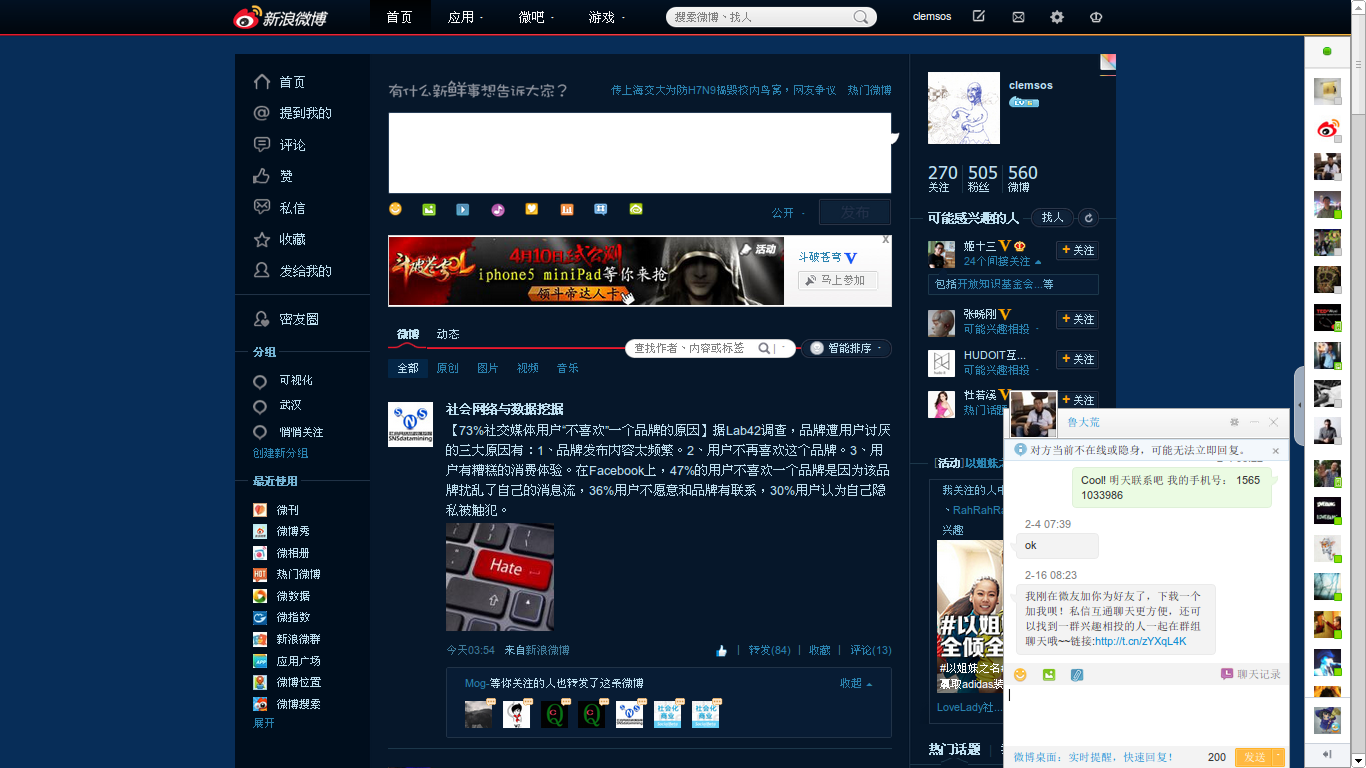
\includegraphics[scale=0.3]{figures/chap1/screenshot.png}
    \caption[Capture d’écran de Sina Weibo]{Capture d’écran de Sina Weibo, réalisé le 9 Avril 2013 à 08:59}
    \label{fig:screenshot_weibo}
\end{figure}

Figure historique de l’Internet chinois, \textit{SINA Corporation} est célèbre pour son portail \url{sina.net} et son immense plate-forme de blogs qui en font le fleuron des fournisseurs de contenus en ligne en Chine. Spécialisée dans ``l’infotainment'' (un mélange très tabloïd d’actualité et de news people), \textit{SINA} est la première compagnie nationale chinoise à avoir été listée au \textit{NASDAQ} dès Avril 2000. Avec son \textit{Weibo}, la firme réussit un coup de force commercial et prouve une fois encore combien la censure gouvernementale est bénéfique à l’industrie du web chinois. Néanmoins, la réussite de \textit{SINA} et de son service de microblog ne se fait pas sans connaître de nombreux ajustements parfois chaotiques. En effet, la stratégie agressive d’acquisition d’audience soutenant la croissance de \textit{Sina Weibo} offre pour garantie aux utilisateurs de pouvoir mieux s’informer et discuter plus facilement en ligne. Dès le début de l’année 2010, les suppressions de comptes utilisateurs et de messages non désirés commencent à se répandre dans le service. Les discussions politiques sont régulièrement effacées et \textit{Sina} se voit contraint de mettre en place un système de censure efficace sous la pression du gouvernement de Pékin. Néanmoins, afin de continuer à garantir la croissance du service, la firme de Pékin laisse une relative liberté aux utilisateurs en étant plutôt souple sur la surveillance des discussions et les actions prises. Des personnalités publiques ou journalistes devenues “weibo-stars” mobilisent régulièrement l’opinion publique autour de sujets d’actualité, attirant souvent des millions de lecteurs et de commentaires. Plusieurs scandales éclatent en ligne, mettant en cause des officiels et leur famille\footnote{Le fils d’un haut-cadre du Parti, arrêté ivre par la police après avoir renversé 5 personnes, annonce : \textit{”Mon père s’appelle Li Gang”} et se voit immédiatement libéré. Cette impunité provoquera un tollé chez les internautes \url{http://www.chinadaily.com.cn/china/2011-03/02/content_12099500.htm}}. Le 23 Juillet 2011, deux trains déraillent sur la ligne reliant Ningbo à Wenzhou inaugurée en fanfare quelques jours auparavant, faisant près de 40 morts et quelques 200 blessés. La colère gronde alors que le gouvernement tarde pendant plusieurs jours à prendre la parole sur ce sujet d’actualité épineux. Sur la toile et \textit{Sina Weibo} en particulier, les discussions vont bon train et les internautes indignés commentent le dernier drame du développement trop rapide de la Chine, où se mêlent détournement de fonds, corruption et sécurité publique. 


\begin{figure}[htbp]
    \centering
    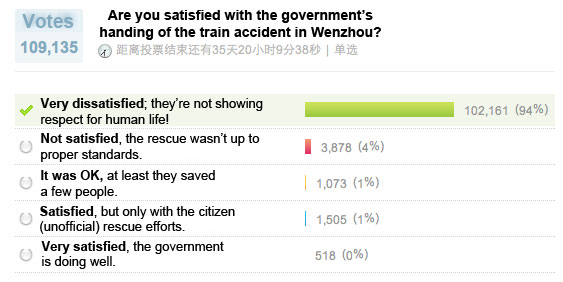
\includegraphics[scale=0.7]{figures/chap1/train.jpg}
    \caption[Sondage Weibo concernant l'accident de train de Wenzhou]{Un sondage publié sur \textit{Sina Weibo} (traduction C. Custer, Tech in Asia, 1 Aout 2011), consulté le 24 Février 2014, à 22h12.}
    \label{fig:poll_weibo}
\end{figure}

\textit{Sina Weibo} désactive alors la fonction de commentaires des messages. Dans les jours suivants, le gouvernement fait enfin une déclaration officielle sur les causes de l’accident de train puis se décide à agir en mettant en garde les internautes trop audacieux de représailles à venir. Les messages controversés sont supprimés, plusieurs comptes d'utilisateurs sont fermés, la police convoque les meneurs des discussions et d’autres mesures d’intimidation sont menées auprès des journalistes et des weibo-stars qui se seraient exprimées un peu trop directement à l’égard du Parti. Dans le même temps, le gouvernement a du mal à se saisir de ce nouvel outil. Alors que les administrations locales, universités et les médias d’État ont plutôt bien réussi le virage de leur stratégie de communication vers le microblog, les membres du gouvernement de Pékin ouvrent des comptes où ils sont parfois raillés, tournés en ridicule et harassés de questions. En Février 2012, les quatre plus grosses sociétés de microblog (dont \textit{Sina Weibo}) annoncent que chaque utilisateur est maintenant contraint de modifier son profil pour mentionner son véritable nom, prénom ainsi que son numéro de carte d’identité. Cette velléité de vérification échoue et est abandonnée quelques semaines plus tard face à la mobilisation des utilisateurs et la difficulté de faire appliquer de telles mesures. Le gouvernement de Pékin édite pourtant une série de règles \textit{“Several Regulations on Microblog Development and Administration Enacted by the Beijing Government”} dont la plus notable sera la possibilité de condamner tous ceux qui auront participé à la diffusion d’informations considérées comme fausses, erronées ou mensongères. Face à la multiplication des actions gouvernementales et à l’apparition d’autres plate-formes, la croissance du nombre d’utilisateurs de \textit{Sina Weibo} est désormais stoppée pour aborder une phase de déclin estimé à près de 10\% dans les deux premiers mois de 2014\footnote{D’après le CNNIC cité dans l’article  \textit{“China’s Twitter is bleeding users”}, 17 Janvier 2014, \url{http://blogs.marketwatch.com/thetell/2014/01/17/chinas-twitter-is-bleeding-users}, consulté le 17 Février 2014 à 18:17}. 

\begin{figure}[htbp]
    \centering
    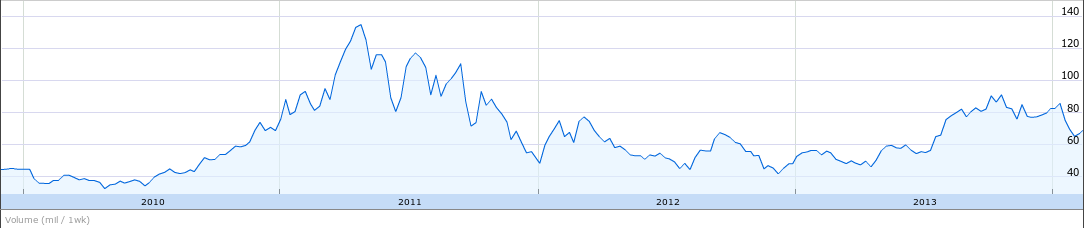
\includegraphics[scale=0.4]{figures/chap1/sina.png}
    \caption[Cours de l’action SINA au Nasdaq entre 2009 et Février 2014]{Cours de l’action \textit{SINA} au Nasdaq entre 2009 et Février 2014 - Source : \textit{Google Finance}, consulté le 17 Février 2014 à 15:28 }
    \label{fig:sina_nasdaq}
\end{figure}

A la lecture de l’histoire de \textit{Sina Weibo} on constate l’ambivalence des actions officielles du gouvernement chinois dans la réussite économique des entreprises d’Internet. Si la firme \textit{SINA} a bénéficié de prime abord d’un avantage compétitif notoire par l’élimination de la concurrence, elle a par la suite souffert des conséquences du contrôle politique de l’Internet, avec notamment une perte de ses utilisateurs.


\subsection[Sina Weibo, un usage plus ludique que \textit{Twitter} ]{Sina Weibo, un usage plus ludique que \textit{Twitter} }

Dans son article nommé \textit{A Tale of two microblogs}, Jon L. \cite{Sullivan2012} raconte comment l’événement historique de la fermeture de \textit{Twitter} en Chine a vu la communautés des microbloggers chinois se scinder en plusieurs groupes distincts : 

\begin{itemize}
\item \textit{Twitter} rassemble une communauté avide de libres discussions, souvent très politisées voire radicalement en opposition avec le gouvernement chinois.
\item \textit{Tencent Weibo} est utilisé par les utilisateurs de \textit{QQ}, typiquement des personnes aux revenus plus faibles accédant au web depuis leurs mobiles.
\item \textit{Sina Weibo} est le favori des travailleurs urbains, souvent plus jeunes ou éduqués, représentant davantage la classe moyenne montante.
\end{itemize}

Dans la littérature en sciences informatiques, plusieurs articles proposent des comparaisons entre \textit{Twitter} et \textit{Sina Weibo}. Une large analyse quantitative et comparative menée avec des jeux de données des deux services \citep{Gao2012} nous apprend que le contenu de \textit{Sina Weibo} est davantage corrélé avec des sentiments positifs (analysés automatiquement). Les utilisateurs de \textit{Sina Weibo} parlent davantage de lieux et de personnes alors que les utilisateurs actifs sur \textit{Twitter} s’intéressent plus aux organisations. Également, \textit{Sina Weibo} connaît un pic d’activité le week-end alors que \textit{Twitter} affiche généralement une baisse de régime dans les fins de semaine. Ces différentes indications suggèrent que \textit{Sina Weibo} serait davantage utilisé pour des activités de loisir quand \textit{Twitter} se destinerait à un usage plus professionnel. Une étude s’intéressant aux tendances sur \textit{Sina Weibo} \citep{Yu2011} indique que la majorité des comptes les plus influents de \textit{Twitter} ont été vérifiés contrairement à \textit{Weibo} où le taux est plus faible chez les grands utilisateurs. La vérification d’un compte se fait par l’authentification auprès du fournisseur de service afin d’attester l'identité de la personne utilisant le compte. C’est un enjeu important pour les figures publiques (marques, stars, hommes politiques, etc.) Cet indicateur nous montre donc l’intérêt professionnel fort entourant \textit{Twitter}, moins pressant dans le cas de \textit{Sina Weibo} où moins de personnes ont ressenti la nécessité de faire officialiser leurs comptes. Sur les deux services de microblog, les utilisateurs inscrits possèdent un réseau de relations identifiables par leur souscription aux fils d’infos d’autres utilisateurs (\textit{follow}). La relation peut être inexistante (\textit{none}), mutuelle (\textit{friend}) ou unidirectionnelle (\textit{follow}, un utilisateur suit un autre mais n’est pas suivi par ce dernier). La comparaison d’échantillons des graphes sociaux issus des deux services \citep{Chen2012} montre comment les relations sur \textit{Sina Weibo} sont plus dissymétriques et moins réciproques, reflétant une hiérarchie plus forte entre les utilisateurs que \textit{Twitter}. 

Un autre facteur important de différentiation entre les deux services est la nature de la diffusion des contenus postés sur \textit{Sina Weibo}. Contrairement à \textit{Twitter} où le texte domine, la majorité des posts de Weibo contiennent des images ou des vidéos \citep{Zhao2012}. Les posts possédant des contenus multimédia (images, vidéos...) sont plus susceptibles d’être diffusés largement et restent en moyenne actifs pour une durée plus longue \citep{Zhao2012}. Également, les contenus sur \textit{Sina Weibo} possèdent une proportion moins élevée de retweets et de commentaires que sur \textit{Twitter} \citep{Zhao2012, Gao2012}. L’activité de la population de \textit{Twitter} est plus intense, moins tournée vers la diffusion de masse et plus réactive aux influx de nouveaux contenus. 

Nous voyons donc que le paysage de \textit{Sina Weibo} se constitue autour de stars et célébrités concentrant l’attention avec des contenus à la diffusion très large. Moins tourné vers l’actualité et la conversation que son homologue \textit{Twitter}, \textit{Sina Weibo} agit comme véhicule de contenus à grande audience, souvent publiés par des personnalités publiques célèbres. Des études quantitatives montrent bien que les contenus les plus échangés et discutés concernent les loisirs et divertissements, la mode, la santé, etc. \citep{Li2013}. Les messages à caractère humoristique (texte, images et vidéos) occupent également une place prépondérante dans les échanges des utilisateurs, contrairement à son homologue américain \textit{Twitter} dominé plutôt par les sujets d’actualité \citep{Yu2011}. \textit{Sina} poursuit ainsi son rôle historique de leader chinois de \textit{l’infotainment}. 

Pourtant, la population de jeunes urbains qui soutient la croissance de son service de microblog reflète aussi les transformations en cours dans la société chinoise. Les journalistes et spécialistes de l’information sont les premiers à se saisir de ce nouveau média. Dans un discours à Stanford en 2013, le PDG de \textit{Sina} Charles Chao explique : 

\begin{quote}
\textit{Le plus grand changement apporté par le microblog en Chine concerne d’abord l’industrie des médias elle-même. Aujourd’hui, plus de 30\% des actualités ont d’abord été reportées sur \textit{Sina Weibo} avant d’atteindre les médias   traditionnels. Le rôle des médias traditionnels a été déplacé vers un traitement des informations en profondeur (in-depth reporting).} \footnote {Charles Chao, PDG de Sina pendant la Stanford Graduate School of Business China 2.0 tenue le 3 Octobre 2013. Disponible en vidéo \url{http://www.youtube.com/watch?v=tlliivJKHk8}, consultée le 19 Février 2014 à 11:23} (traduction de l’auteur)
\end{quote}

L’omniprésence des supports mobiles (smartphones, tablettes)\footnote{Selon l’Universal Telecommunication Union, \textit{``la Chine dépasse 1 milliard d’abonnements mobile, avec 400 millions d’utilisateurs d’Internet mobile dépasse ainsi les États-Unis comme leader du marché des smartphones''}, \url{http://mobithinking.com/blog/china-top-mobile-market} consulté le 24 Février 2012.} permet en effet des modes de traitement de l’information jusqu’ici inconnus qui bousculent les hiérarchies très contrôlées des salles de rédaction chinoises. Alors que la population urbaine croît rapidement, le smartphone est \textit{``the first big urban purchase''} \citep{Wallis2013} pour les nouveaux arrivants en ville et représente un outil indispensable de participation à la société. En 2008, la Chine était le seul pays en Asie où les moins de 30 ans possèdent plus d’amis en ligne que hors ligne \citep{Hinckley2009}. Ainsi, les réseaux sociaux jouent un rôle primordial dans la socialisation urbaine et viennent changer les modes d’expression. Le lectorat chinois a perdu toute confiance dans la plupart des médias traditionnels suite à l’absence répétée de courage et à la rétention d’informations cruciales dans les dossiers importants animant le pays. 

Le microblog s’installe comme une nouvelle source de confiance pour des millions de citoyens voulant comprendre et prendre part aux changements cruciaux de la société chinoise moderne. Un rapport de l’Institut de Journalisme Reuters à l’Université Oxford paru en 2013 montre comment les usages du microblog ont amené des transformations dans le quotidien des journalistes chinois. Le journalisme d’investigation a notamment connu un essor important grâce au renouvellement des sources et une large diffusion en ligne des sujets. \textit{Sina Weibo} n’a pas amélioré nécessairement la qualité de leurs investigations, mais a par contre permis une plus grande dissémination. Il est à noter que les spécificités de l’écriture chinoise rendent possible l’écriture d’un court texte en 140 caractères, alors qu’une telle longueur autorise seulement une courte phrase dans une écriture utilisant un alphabet latin. La mobilisation des utilisateurs pour la protection des journalistes a également joué un rôle important ainsi que le renforcement de procédés de vérification existant depuis longtemps sur les forums du web chinois. Très populaire dans les années 2000, Le \textit{``moteur de recherche de viande humaine''} (\textit{renrou sousuo}) est une forme de traque d’individus en ligne réalisée par un large nombre d’internautes à partir d’un nom ou d’une photo. Il s’agit souvent de retrouver quelqu’un désigné comme ``coupable'' (d’adultère, de corruption, etc) en réunissant un maximum d’informations à travers la Toile afin d’identifier ou de localiser la personne. Devant les dérapages rapides de ce type de procédés, les questions d’éthique sont au cœur des discussions qui entourent le journalisme en ligne. En effet, l’usage des médias sociaux a permis à certains journalistes de faire pression sur les pouvoirs publics, amenant parfois à la censure de leurs travaux, mais a également permis une très large auto-promotion pour de nombreux journalistes devenus des stars de \textit{Weibo}.

\begin{figure}[htbp]
    \centering
    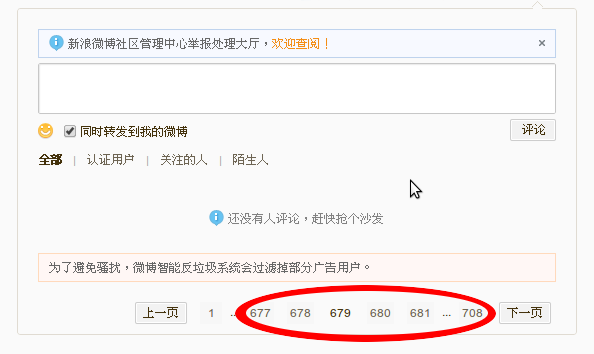
\includegraphics[scale=0.5]{figures/chap1/comments.png}
    \caption[Commentaires supprimés par Sina]{La trace des commentaires supprimés par Sina est encore visible - Page 677 à 708, les commentaires ont été supprimées, soit approximativement 4\% messages supprimés (589 messages sur 13452, à raison de 18 à 20 messages par page). Capture d’écran effectuée le 29 Janvier 2013 à 12:32:42, \url{http://www.weibo.com/1701401324/zeoBquVKi}, consulté le 16/02/2013.}
    \label{fig:comments}
\end{figure}

Le contrôle des contenus sur \textit{Weibo} est donc une réalité quotidienne et a été depuis son lancement la source de plusieurs études. Les formes les plus courantes sont : la suppression de posts, la suppression de comptes utilisateurs et le blocage de mots-clés. Le blocage de mots-clés s’effectue dans le moteur de recherche interne du site (“pas de résultats” quand vous cherchez un mot bloqué) et plus récemment par l’impossibilité de poster un message contenant des mots ou des adresses web bloqués \citep{Ng2013}. La pratique de la suppression de comptes s’est intensifiée en 2013\footnote{ \textit{“Over 100,000 \textit{Sina Weibo} Accounts Shut Down or Penalized for Govt Rules Violations”} par Gabriela Vatu, 14 November 2013 \url{http://news.softpedia.com/news/Over-100-000-Sina-Weibo-Accounts-Shut-Down-or-Penalized-for-Govt-Rules-Violations-400289.shtml} consulté le 17 Février à 16:42} avec notamment la suppression de millions de “zombies” présents sur le site. Les “zombies” sont des comptes utilisateurs créés par des robots dans le but de reposter automatiquement des contenus et d'augmenter le trafic sur le site. Les exigences des annonceurs publicitaires de plus en plus présents sur le site ont obligé \textit{Sina Weibo} à faire la chasse aux robots sur son site, faisant ainsi diminuer le nombre de comptes actifs de manière significative. La firme Sina est garante auprès du Ministère de la Sécurité Publique chinois des contenus qu’elle diffuse et effectue à ce titre une surveillance constante pour supprimer les messages “non-conformes”. Lors de nos recherches, nous avons constaté que l’interface de \textit{Sina Weibo} garde la trace des commentaires supprimés par le système d’administration. Dans les messages supprimés se trouvent à la fois des posts d’utilisateurs “zombies” et les posts jugés incorrects par les administrateurs. Au total, la suppression des messages s’effectue avec un taux estimé à environ 16\%, allant jusqu’à plus de 50\% dans certaines provinces comme Ningxia ou le Tibet contre seulement 12\% à Beijing \citep{Bamman2012}.


\section[Code, langage et milieu(x) numérique(s)]{ Code, langage et milieu(x) numérique(s)}

L’espace d’expression offert par l’Internet chinois et ses services de réseaux sociaux héberge donc une variété de pratiques, de questions et de réflexions qui nécessitent d’être appréhendées avec des outils de problématisation et d’analyse spécifiques. Dans la troisième et dernière partie de ce chapitre introductif, nous allons donc nous pencher sur les concepts existants dans la littérature scientifique sur l’existence \textit{in situ} des objets numériques. Afin de mettre en perspective le Web chinois et l’histoire de ces objets, nous introduirons notamment le concept de \textit{milieu numérique}, héritier de l’idée complexe de milieu que nous explorons ci-après.

\subsection[Lieu, espace, territoire et technologies]{Lieu, espace, territoire et technologies}
Géographie, management et diffusion de l’innovation, histoire des technologies, \textit{cultural studies} ou études “nationales”, les travaux qui s’intéressent aux relations entre technologies, espace, lieux et territoires sont nombreux et offrent un paysage riche où se croisent de nombreuses disciplines scientifiques. L’influence des réseaux de transports sur l’expérience humaine et le développement des villes a notamment été largement étudiée \citep{Offner1993,Doulet2001}. L’Internet a également fait l’objet de nombreuses études monographiques (par pays) ou comparatives, une étude à l’échelle mondiale présentant en effet des problèmes de données et évidemment d’échelle \citep{Dupuy2004}. En Chine où l'urbanisation produit actuellement une vaste migration des ruraux vers la ville, l'utilisation des réseaux sociaux médiatise bien souvent les choix de lieux et les rencontres des nouveaux arrivants. De nombreux groupes de discussions réunissent par exemple les nouveaux acheteurs d’immobilier qui échangent leurs stratégies d’achat et de défense de leurs droits et de leurs biens \citep{Li2013}. L’usage des réseaux sociaux revêt pour les nouveaux arrivants une importance capitale, notamment dans la recherche de groupes similaires et l’échange d’expériences. A travers le navigateur, ils s'approprient la ville étrangère pour s'en construire peu à peu une représentation à leur image.

La carte notamment joue sur le web un rôle important d’abord en tant qu’illustration, puis plus récemment d’interface avec le réel. Loin d’être figée par le territoire, la carte le décrit sous un ou des angles particuliers \citep{Brunet1987, Jacob1992}. Le développement de standards comme le système GPS \citep{Haklay2008} et de services et outils de cartographie ont contribué à une appropriation de la pratique cartographique par un nombre croissant de personnes \citep{Crampton2009}. De nouvelles formes de données produites par les utilisateurs parfois appelées \textit{``volunteered geographic information''} \citep{Elwood2008} utilisent les services en ligne comme Google Maps pour dessiner un \textit{``miroir du monde offline''} \citep{Graham2011}. Le courant dit de la néogéographie fait usage du GIS et des outils en ligne (Google Maps, Flickr, etc.) pour comprendre les pratiques de ces nouvelles formes de \textit{``géographies volontaires''} \citep{Turner2006}. Ce rôle croissant de la cartographie dans l’usage d’Internet produit un \textit{``Geoweb''} constitué de données et métadonnées spatiales \citep{Crampton2009}. Le point d'entrée unique qu'offre le marqueur spatial (\textit{geotag}) réunit souvent de vastes quantités de données disparates: Open Data territorial, géo-localisation, GIS, POI\footnote{GIS : Geographic Information System ; POI : Point-Of-Interest}, etc. \citep{Torrens2010}. Cette présence accrue dans le réseau dessine l’enjeu non seulement de cartographier le monde, mais également de cartographier le réseau lui-même, ouvrant ainsi de nouvelles voies pour découvrir la construction sociale des espaces par des pratiques individuelles et de groupe. Dans cette étude, nous avons donc choisi d’interroger les objets numériques afin de comprendre comment se structurent la parole et la conversation dans le contexte unique de l’Internet chinois. Afin d’articuler les multiples dimensions d’analyse qui viennent enrichir notre réflexion, il nous faut donc brosser un portrait en large de l’Internet chinois, en le considérant tour à tour comme un \textit{espace} structurant pour les actions des internautes qui le pratiquent, comme un \textit{territoire} sujet aux relations de pouvoir actualisées par les groupes et individus et enfin comme un \textit{lieu} habité par ceux qui y construisent chaque jour des significations communes. Nous proposons ici une revue sélective des quelques travaux à même de nous apporter des éclairages pertinents dans la vaste littérature s’intéressant aux dimensions géographiques des TIC.

\subsubsection[Code / space : l’espace transductif des TIC]{Code / space : l’espace transductif des TIC}

Dans leurs recherches autour de la géographie des technologies numériques, Dodge \& Kitchin ont travaillé à développer le concept de code comme un élément fondateur des espaces modernes dans lesquels nous évoluons. Reflétant l’importance croissante accordée aux TIC dans l’environnement urbain, ils citent un travail sur la production automatique des espaces : \textit{“De plus en plus, les espaces de la vie  quotidienne nous parviennent chargés de logiciels (software)”} \citep{Thrift2002} En effet, si le projet urbain a été guidé pendant le demi-siècle dernier par l’apparition de la technologie automobile dans l’espace des rues, les TIC paraissent prendre le relais avec l’idée d’une ville intelligente et connectée, connue sous le nom de \textit{`` smart city ''} \citep{Ascher2009,Picon2014}. Dodge \& Kitchin ont donc fait du \textit{code} une des pierres d’angles de l’appréhension de l’espace dans leur travail en le définissant comme suit : 

\begin{quote}
\textit{``an instruction or rule that has a single outcome determined by a binary logic (yes/no). The combination of these indidivuals logic rules produces code (program).''} \citep{Kitchin2011}.
\end{quote}

La part croissante des TIC dans nos espaces quotidiens amène les auteurs à envisager l’espace dans son interaction avec le code, symbolisant la suite d’instructions machiniques et électroniques qui permettent à un espace de remplir sa fonction. Dans un article intitulé \textit{Flying through code/space: the real virtuality of air travel}, Dodge \& Kitchin analysent la structure des espaces aéroportuaires. De l’achat des tickets jusqu’au vol des avions en passant par la gestion des bagages, le bon fonctionnement d’un aéroport est entièrement régi par les longues successions d’instructions du code. Ici, Dodge et Kitchin proposent le concept de code/space pour décrire ce type d’espace spécifique où lorsque le code échoue (\textit{failure}) alors le code/space tout entier échoue \citep{Dodge2004}. L’exemple de l’aéroport est parlant : si le système de check-in des bagages ou les machines responsables du contrôle de sécurité des passagers ne fonctionnent pas, alors l’espace aéroportuaire ne peut exister en tant qu’aéroport. L’analyse de la spatialité ne se situe alors plus dans un domaine sémantique ou narratif, mais plutôt dans les processus et opérations qui s’y déroulent et le code et les technologies y jouent un rôle primordial : 

\begin{quote}
    \textit{``Code is employed as the solution to a problem, a particular kind of transduction  is occurring.''} \citep{Kitchin2011}. 
\end{quote}

L’espace n’est pas un donné mais s’explique plutôt comme : \textit{``une forme d’ontogenèse (en perpétuel devenir-au-monde), l’espace est une pratique; un faire ; un événement (…) qui ne pré-existe pas à son faire (doing)''} \citep{Kitchin2011}. L’espace est considéré non pas comme une production, mais comme une \textit{transduction}. Reprenant le travail de Simondon sur l’individuation par la technologie, Dodge et Kitchin présentent l’espace comme une pratique qui comprend les actes, actions, occurrences, mémoires, perceptions, etc. d’un groupe d’individus s’y trouvant. La fonction de l’espace est structurée par les individus et le code y est considéré comme une entité agissante. Dans le \textit{code/space}, la relation dyadique entre code et espace est bijective: l’un ne peut aller sans l’autre. En terme simondonnien, la transduction ne peut être assurée sans code. Si l’exemple de l’aéroport illustre bien cette nécessité du code dans le devenir-espace, Dodge et Kitchin ont également identifié d’autres catégories où cette relation est plus ténue : les \textit{coded spaces}, qui peuvent poursuivre leurs fonctions même lorsque le code échoue ; les \textit{background coded spaces} où les processus de transduction induis par l’espace ne s’appuient pas nécessairement sur le code, mais proposent néanmoins des possibilités de l’activer (machine éteintes ou inactives, etc.) 

L’analyse fonctionnelle des rapports entre espace et technologie de Dodge \&Kitchin montre comment les TIC peuvent être un facteur \textit{transductif} pour les individus se mouvant dans les espaces de leurs vies quotidiennes. Si nous appuyons pleinement ce constat, il nous semble que le parti-pris des auteurs de considérer le “code” comme une abstraction incluant uniquement les instructions ou “logiques machiniques“ ferme la porte à l’immense densité des activités symboliques qui se jouent dans l’usage des technologies. Comment notamment considérer les “contenus” du web dans cette grille de lecture? Comment resituer dans une perspective historique les logiques de médiation de l’espace par les technologies de l’écriture? Il nous semble en effet que la faillite fonctionnelle (\textit{failure}) des code/space précède l’arrivée des technologies et s’opère déjà à un niveau symbolique - la fonction de l’espace du Palais du Louvre après la chute des rois de France se voit radicalement modifiée. La transduction opérée lors de la pratique d’un espace s’effectue dans un jeu d’appropriation symbolique qui passe notamment mais pas seulement par les technologies. Les technologies du langage et de l’information jouent notamment un rôle crucial dans l’affirmation du récit symbolique (\textit{narrative}) qui construit l’espace. L’activité du code dans la structuration des code/space de Dodge \&  Kitchin existe sous une forme non seulement fonctionnelle mais également sémantique, voire phatique ou même esthétique comme l’a décrite Jakobson dans ces analyses des fonctions du langage \citep{Jakobson1956}. Au-delà de sa dimension machinique, le code possède les caractéristiques d’une \textit{poiesis} dépassant l’idée simple de fonctionnalité pour exister dans la complexité d’une écriture comme traduction du langage humain et machine.

\subsubsection[Codes, discours et territoires des technologies]{Codes, discours et territoires des technologies}

Le code serait davantage à comprendre comme un mode d’expression humain à travers la technologie, actualisant l’\textit{épistémè} décrit par Foucault dans \textit{Les Mots et Les Choses} comme élément fondamental de la pensée d’une époque et sa considération pour le monde \citep{Foucault1996}. \'Etat des connaissances scientifiques et littéraires, l'épistémè existe comme somme des savoirs d’une époque, présupposée traduite en un regard sur le monde. Le \textit{code} exprime les savoirs d’aujourd’hui dans de nombreux langages écrits. Le code source d’une page Internet, d’un programme informatique ou d’un driver hardware ne s’écrit pas seulement en langage ``machine'' mais fait appel à plusieurs langages informatiques et humains. A la fois production savante, outil scientifique, vecteur d’expression et interface des savoirs, le code constitue l’expérience narrative du monde par les TIC. Possédant de nombreux mots, aspects et syntaxes issus de multiples langues humaines, les replis de l’écriture informatique laissent transparaître de tout bord leur origine littéraire. L'alphabet se voit augmenté de nombreux caractères qui le rendent compatible avec l’encodage des bases de données - pensons à l’Unicode notamment \citep{Guichard2014}. Rappel à l'ordre, l'arrêt soudain de l’ordinateur ou la perte d’un fichier nous laisse frappés d’illettrisme. Seuls une minorité de personnes ``lettrées'' de l’informatique peuvent déchiffrer et comprendre le ``bug''. Ainsi, la définition du ``code'' de Dodge \&  Kitchin doit être étendue pour recouvrir plus largement les pratiques symboliques liées aux activités de l’écriture du code dans ces espaces.


Le code ainsi redéfini nous ramène alors à une lecture foucaldienne du discours dans sa relation intime avec le territoire \citep{Foucault2004}. Dans ces nombreux travaux sur la généalogie, Michel Foucault cherche à comprendre comment les relations de pouvoir créées par les discours portés sur les objets président à la production de territoires et d’interdits comme autant de sujets de ces discours. Nous définissons la \textit{discursivité} comme le processus de construction de ces discours. Historiquement, l’Internet a été très tôt sujet à l’appropriation par le discours de nombreux groupes actifs dans une volonté de territorialisation. La métaphore géographique et spatiale a structuré le vocabulaire de l’Internet dès sa création \citep{Graham1998}: site, cyberspace, etc. L’\textit{Electronic Frontier Foundation} se charge de protéger l’u-topie qu’est Internet avec sa fameuse \textit{Déclaration d’Indépendance du Cyberespace} \citep{Barlow2001}. A l’opposé du spectre, les autoroutes de l’information in-forment le paysage comme autant de géogrammes massifs \citep{Berque1999}. L’appropriation des protocoles du réseau, notamment par la lutte pour le respect de standards ouverts ou partagés, s’ancre également dans les pratiques du discours. Les mots \textit{free} et \textit{open} cristallisent l’histoire des revendication territoriales de l’Internet \citep{Blondeau2000}. L’autre grande métaphore constitutive de l’Internet est textuelle avec ses pages, langages et hypertextes \citep{Vandendorpe1999}. La formule choc \textit{``Code is law''} \citep{Lessig2006} résume l’idée  que les processus textuels du code mettent en jeu un ensemble de rôles, protocoles et mises en scène qui agissent comme autant d’autorités à travers le discours. La jurisprudence fait loi, comme écrit sur les murs des bureaux de \textit{Facebook} à Palo-Alto : \textit{``Code wins arguments''} \footnote{Phrase mentionnée dans la lettre écrite par M. Zuckerberg aux investisseurs lors de l’IPO de \textit{Facebook} \url{http://www.sec.gov/Archives/edgar/data/1326801/000119312512034517/d287954ds1.htm\#toc287954_10}}. La territorialisation de l’Internet se fait ainsi au travers d’un ensemble de pratiques discursives, méta-grammaire des discours en ligne. La confrontation symbolique au sein des territoires numériques se poursuit dans le discours, réifié dans les pratiques du code.

Sur l’Internet chinois, les pratiques de censure de l’écriture en sont le reflet le plus frappant. Blocage de mots-clés, détournements de langage, suppression et modification de texte sont l’expression de cet affrontement de discursivités parfois antagonistes. La Grande Muraille gouvernementale scanne les masses de texte pour reconnaître et stopper des mots tels que \textit{``Printemps arabe''} ou \textit{``évènements de Tian-An Men''} \citep{MacKinnon2012}. Néanmoins, l’état actuel des techniques de \textit{data mining} ne permet pas encore de déceler les phénomènes langagiers comme les jeux de mots ou l’ironie. Bien souvent, les internautes chinois choisissent l’humour pour permettre à leurs idées de se frayer un chemin. Revêtant leurs masques de chat, les internautes chinois sont devenus spécialistes dans la publication de jeux de mots, chansonnettes et petites vidéos d’animaux, comme autant de couperets cinglants pour railler les officiels trop pompeux de Pékin. Dans la guerre de l’information que se livrent sans cesse censeurs et internautes, de simples photos truquées de crabes et de lamas peuvent devenir héroïques. Ces blagues numériques, d’apparence inoffensive, font chaque jour le tour de la Toile chinoise, portant en elles toute la subversion d’internautes aspirant à plus de liberté. Début 2010, alors que pleuvaient les longs discours pieux du Parti sur l’harmonie de la nouvelle société (en chinois \textit{hexie}), on voit apparaître en ligne des essaims de crabes de rivière (se prononçant également \textit{hexie}) couverts de chaînes en or criant : \textit{“Vive l’harmonie”} au volant de leur limousine. Devenus aujourd’hui une image de la corruption des hauts dignitaires du Parti, on croise régulièrement dans les commentaires d’un article officiel un petit crabe de rivière, tel un rapide rappel posté par un lecteur.


\begin{figure}[htbp]
    \centering
    \subfloat[(hexie) : Harmonie / Discours du PCC sur l’harmonie]{ 
        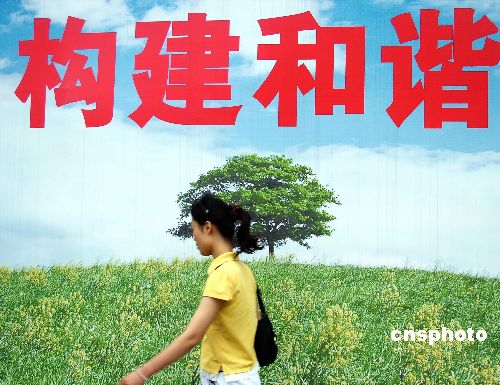
\includegraphics[scale=0.37]{figures/chap1/hexie2.jpg} 
    }
    \subfloat[(hexie) : Crabe de rivère / Mème satirique]{ 
        
\includegraphics[scale=0.37]{figures/chap1/hexie.jpg} 
    }
    \caption[Hexie, les crabes de rivières]{ \zh{和谐} VS \zh{河蟹} - Mot de la semaine : Crabe de Rivière - China Digital Times du 21 Mars 2012 - Licence Creative Commons \url{http://chinadigitaltimes.net/2012/03/word-of-the-week-river-crab}, consulté le 15 Février 2013.}

\label{fig:hexie}
\end{figure}

On voit bien comment le code décrit un territoire sujet à l’autorité politique sous la forme d’un système de \textit{data mining} cherchant à mettre en forme le discours. La fonction du \textit{code/space} sémantique que forme ici l’espace de l’Internet est réécrit par un jeu de langage. La circulation d’objets digitaux permet de reterritorialiser cet espace en apparence régi par un code strict de censure. 

\subsubsection{Les lieux des technologies}
Dans son célèbre livre sur les Arts de Faire, \cite{Certeau1980} considère la ville comme un texte dont chaque piéton énonce et révèle (\textit{performe}) des sens nouveaux par son activité de marcheur. Actualisant l’espace urbain par sa marche, l’habitant de la ville s’approprie des lieux restant néanmoins partagés avec d’autres. Au détour des rues, le sens commun des lieux urbains se construit avec les multiples énonciations de ceux qui les habitent et les font vivre. Cette magnifique image de la poésie du texte urbain met en lumière la dualité que nous avons abordée précédemment : l’espace ne peut fonctionner sans les pratiques de ses habitants. Plus encore, l’être-ensemble et le devenir-soi procèdent de la construction de lieux communs, \textit{poiesis} des espaces habités. Les TIC font aujourd’hui souvent partie intégrante des lieux que nous habitons. \cite{Graham1998} dans son travail sur l’étude des lieux et de leur rapport à la technologie identifie trois types majeurs d’approches dans la littérature :


\begin{enumerate}

\item L’approche \textit{``substitutive''} ou \textit{``transductive''} qui voit dans l’arrivée des TIC la disparition de la valeur des lieux : un idéal de proximité utopique \citep{McLuhan1962} ou un discours dystopique sur leur proche disparition \citep{Virilio1998, Auge1995}. Ces considérations sont les formes traditionnelles du débat accompagnant l’innovation dont sont férus la communication industrielle et la critique des médias \citep{Ramonet2001}, restant souvent purement prospectif et faisant peu de cas des usages.

\item Plus modérée, l’approche qualifiée par Graham de \textit{``co-évolutionniste''} s’interroge sur la façon dont les interactions dynamiques des espaces virtuels (\textit{space of flows}) et réels (\textit{space of places}) \citep{Castells2009} produisent de nouveaux lieux . Ces études économiques et sociales prennent la forme d’une médiologie de l’espace adaptée aux études stratégiques pour l’urbanisme et l’implantation des télécommunications. Son interprétation par les aménageurs lui donne parfois une dimension déterministe peu utile à la compréhension des phénomènes liés à l’appropriation et l’historicité des technologies \citep{Offner1993}.

\item Une dernière approche plus récente se cristallise autour de l’idée de relations et de réseaux. Afin d’éviter l’écueil des causalités directes et de la notion fataliste d’impact, les lieux sont présentés comme \textit{`` des moments articulés dans un réseau de sens et de relation sociales ''} \citep{Massey1993}, des assemblages entre objets matériels “actants” \citep{Latour1996}, individus et groupes sociaux. Cette approche s’intéresse davantage au lieu comme une géométrie sociale en mouvement, liée au temps et à la situation \citep{May2001} et refuse l’idée d’une existence “virtuelle” commune à différents objets \citep{Bingham1996}.

\end{enumerate}

En privilégiant une approche dynamique et relationnelle des lieux comme constructions sociales de sens \citep{Kyle2007}, la technologie perd son rôle déterministe de productrice d’espaces et d’usages pour devenir une actualisation d’un espace-temps géographique et historique par des groupes d’individus. Comme le note Cresswell dans son travail sur les lieux : \textit{“places are practiced. People do things in place.”} \citep{Cresswell2004}. Il propose trois aspects pour décrire l’actualisation des lieux par leurs pratiques : location (un point dans l’espace, \textit{“the ‘where’ of place”}), \textit{locale} (les aspects visibles et tangibles du lieu, \textit{“the way a place looks”}) et \textit{sense} (\textit{“the feelings and emotions a place evokes”}). Néanmoins, cette définition ne permet pas d’appréhender l’existence des lieux en ligne (le site web d’un lieu est-il une \textit{locale} ou une partie du \textit{sense}?). Graham et Zook propose le concept de DigiPlace : \textit{`` DigiPlace - that is, the use of information ranked and mapped in cyberspace to navigate and understand physical places (…) In other words, DigiPlace represents the simultaneous interaction with software (information) and `hard-where' (place) by an individual.''} \citep{Zook2007}. S’inspirant des travaux de Harley sur le pouvoir du cartographe, leur travail sur le rôle de Google Maps dans la présence des lieux sur Internet met à jour l’interaction et l’hybridation entre existence spatiale et existence en ligne constituant les DigiPlace. 

Les phénomènes de transduction à l’œuvre dans les pratiques spatiales de l’Internet sont donc le reflet des états du réseau à un moment donné. Les lieux eux-mêmes forment ainsi un réseau basé sur leurs relations et similarités. Brunet dans son \textit{Vocabulaire de la Géographie} propose notamment l’idée de synapses: \textit{``espaces ou lieux par lesquels on passe, par où l'on communique, les isthmes, les détroits, les estuaires, les carrefours, les ports et les ponts, etc.;''} \citep{Brunet1972}. Envisagés par leur fonction ``synaptique'' , les lieux deviennent alors un construit social au rôle clair, évitant l’écueil d’une qualification en-soi. Aéroports, hypermarchés, aires d’autoroutes ou zones industrielles ont été qualifiés de \textit{non-lieux} par Marc Augé, produits d’une  hyper-modernité \textit{`` qui ne peut se définir ni comme identitaire, ni comme relationnel, ni comme historique. ''} \citep{Auge1995}. Réfutée plus tard par l’auteur lui-même, cette idée de lieux simplement \textit{produits}, et non construits fait l’impasse sur la tension d’usage, le devenir lieu que modèlent ses utilisateurs assidus ou épisodiques, ceux qui y travaillent voire même y habitent. Le lieu n’est pas nécessairement “patrimonial” comme produit d’une histoire, mais peut \textit{`` être ou ne pas être un non-lieu selon le statut de l'individu envisagé. ''} \citep{Debarbieux1993}. Les hypermarchés et leurs galeries marchandes sont des haut-lieux de socialisation et de rencontres pour les adolescents vivant en banlieue \citep{Matthews2000} mais paraissent froids et inhumains aux habitants des rues du centre-ville.

L’étude menée par Puel, Pons et Xiaoting autour des pratiques sociales environnantes les cafés Starbucks de Beijng (Chine) montre également comment la stratégie marketing de la firme s’appuie précisément sur cette “absence patrimoniale” pour faire sa place au travers du vaste territoire chinois. La non-existence d’un \textit{“bon café avec Internet”} dans les villes chinoises offre la possibilité aux usagers de ces cafés récemment apparus de s’y rendre pour utiliser l’Internet ou retrouver leurs amis \citep{Puel2007}. Ainsi, l’absence d’histoire n’interdit pas la constitution de pratiques communes à forte valeur symbolique se comprenant ici dans des réseaux d’appartenances mondiaux (jeune, dynamique, urbain, etc.). Dans son livre \textit{The Great, Good Place}, Ray Olenburg propose le concept de tiers-lieu pour décrire ces lieux qui, séparés de l’environnement de travail ou de la maison, permettent de se socialiser. Jouant un rôle majeur dans la construction de communautés et la constitution d’une société civile, ces tiers-lieu doivent répondre à certains critères comme: un cout d’accès nul ou modeste, une très bon accessibilité, la présence régulière des \textit{``habitués''}, un lieu accueillant et confortable et enfin un lieu où l’on peut rencontrer facilement de nouvelles personnes \citep{Oldenburg1999}. Ces tiers-lieux forment donc avant tout un réseau de lieux défini par les usages. L’idée de tiers-lieu virtuels a également été mentionnée pour désigner les chatrooms ou les plate-formes de réseaux sociaux en ligne remplissant des fonctions sociales similaires \citep{Soukup2006}.

Nous voyons donc qu’en considèrent les lieux de l’Internet, nous mettons à jour un ensemble de pratiques ne s’intéressant plus nécessairement à l’ordre du discours (et aux pratiques de censure notamment) mais plutôt aux phénomènes d’individuation, notamment au travers des multiples actes d’énonciation qui forment les pratiques et usages du web. Dans cette étude nous cherchons donc à comprendre de manière plus profonde comment les internautes habitent leur Internet. Il ne s’agit pas d’analyser le discours en termes de relations de pouvoir mais plutôt d’essayer de distinguer comment les circulations des objets numériques structurent les pratiques des internautes, comme autant de lieux habités quotidiennement.

\subsection[Le milieu : richesse et désuétude ]{Le milieu : richesse et désuétude }

Afin de problématiser les relations entre protocoles du discours et pratiques locales d’appropriation, nous avons choisi d’introduire le concept de \textit{milieu numérique}. Nous définirons d’abord brièvement ce concept avant de présenter un regard historique sur l’idée de milieu en science. Nous discuterons ensuite de l’acception particulière que nous avons choisie de défendre ici et nous verrons comment cette notion sera utile pour la suite de notre étude sur les réseaux sociaux en Chine.

L’idée de milieu numérique est a priori définie dans les termes suivants:

\begin{quote}
    \textit{``The multiple networks, which are connected by protocols and standards, constitute what I call a digital milieu.''} \citep{Hui2012}
\end{quote}

L’usage de multiples interfaces et le dédale des réseaux TIC constituent \textit{``un nouveau milieu perceptif''} \citep{Barboza2006}. Notre milieu physique est aujourd’hui (déc)ouvert par l’existence de notre milieu digital qui nous aiguille. Rencontres, restaurants et voyages sont souvent d'abord médiatisés par l’Internet. Ainsi, nous évoluons dans un milieu numérique agissant comme support de processus de transduction et de connaissance du monde. Le code prend ici pleinement part à la construction de ce milieu digital, à la fois déterminant pour la production des actes de discours et ouvert à l’appropriation des pratiques et usages du quotidien.

Historiquement, le concept de milieu se détache du centre pour resituer et mettre en perspective la relation des êtres à leurs environnements sous des jours parfois contradictoires. Débattue puis écartée mais toujours très usitée, la notion de milieu introduit autant le déterminisme d’un combat pour la survie et l’adaptation, que la liberté créatrice du sujet dans un univers ouvert à sa volonté. 

Pour illustrer au mieux la fécondité philosophique de la notion de milieu, nous allons tout d’abord essayer de comprendre la trajectoire de ce mot durant les siècles derniers \citep{Canguilhem1965}. Sans remonter à son aube étymologique, nous nous apercevons que le mot milieu décrit un trajet singulier dans le monde des sciences. Employé dès le XVIème siècle par Descartes dans son \textit{Traité de la lumière}, il représente pour Newton une mesure de distance dans l’éther, cette non-matière  structurant la gravitation qui fait se mouvoir les objets. Défini plus tard par d'Alembert dans son encyclopédie comme un : \textit{"espace naturel dans lequel un corps est placé, qu'il se meuve ou non"}, le mot connaîtra durant tout le XIXème un large développement sémantique en s'étendant de la physique à la biologie. Les naturalistes français de l’époque affirment que le milieu n’est pas seulement \textit{environnant} mais influe sur les êtres vivants. Ainsi Lamarck dès 1809 écrira dans sa \textit{Philosophie Zoologique}: \textit{"le milieu a une grande puissance pour modifier les organes"}. 

Le XIXème siècle est un moment marquant pour ce concept et structurant pour l’histoire des sciences dans son ensemble \citep{Taylan2010}. Auguste Comte, inspiré de la biologie, articule le vital au social dans la sociologie naissante et décrit le milieu comme \textit{``l’ensemble des circonstances extérieures (…) nécessaires à l’existence de chaque organisme déterminé''} \citep{Comte1838}. Comte introduit une première dialectique des rapports avec le milieu comme conditions de possibilité de la vie: \textit{``Tout être vivant (…) modifie sans cesse son milieu.''}, écrit-t-il alors. Le concept connaît un succès croissant en France et les penseurs d’Outre-Rhin se le réapproprient en lui donnent un sens différent. S’opposant au francisé \textit{Der Milieu}, le géographe Ratzel introduit dans son \textit{Anthropogéographie} (1899) le terme \textit{Umwelt}. Ce mot se démarque rapidement par sa dimension fortement déterministe. Dans un même mouvement, le physiologiste et biologiste Jakob von Uexküll étudie dans son laboratoire la tique et se rend compte que le milieu de la tique se définit non pas par tout l’environnement qui l’entoure mais seulement par ce qui lui est utile et approprié. Le milieu devenu \textit{Umwelt} s’oppose alors à l’environnement indifférencié et devient l’ensemble des éléments porteurs de significations (\textit{Merkmalträger}) pour un être. Uexküll propose ainsi une \textit{``biologie subjective''} étudiant les relations de chaque espèce avec son milieu. Dans l’Allemagne du siècle débutant, Uexküll diffuse largement sa théorie qui ne s’adresse pas tant aux animaux qu’à l’humain dont le milieu serai la Patrie (\textit{Heimat}) \citep{Feuerhahn2009}. Reflétant les débats guerriers entre la \textit{Kultur} allemande et la \textit{Civilisation} française \citep{Elias1975}, l’idée de Milieu cristallise la tension politique sur les relations entre nature et vivant qui déchirera l’Europe pendant longtemps encore. Foucault dans son cours au Collège de France du 11 Janvier 1978 parle de l’influence de l’idée de milieu sur la conception du territoire pour les urbanistes du XVIIIème siècle. Sous Louis XIV, les villes sont encore construites dans un espace conçu comme vide (voir \textit{Richelieu} en Indre-et-Loire). A l'inverse, la question de l’urbaniste du XVIIIème est de comprendre la ville dans son évolution future. L’enjeu est devenu l’\textit{adaptation} du milieu existant (à la fois urbain et naturel), la transformation du \textit{donné} compris comme un élément qu’on peut venir modifier. L’idée sous-jacente de milieu ouvre la possibilité de l’appropriation de la nature. En terme foucaldien, cette nouvelle bio-politique se fonde sur la territorialisation du milieu comme nouveau centre des enjeux de pouvoir. L’ère industrielle réalise ce projet d’une adaptation à la fois \textit{au} et \textit{du} milieu vu comme tension nécessaire de l’évolution, passage obligé vers la civilisation. Alors que l’humain est placé dans son rôle central par l’astronomie galiléenne puis l’évolution darwinienne, l’idée de milieu pose comme enjeu majeur du vivant la maîtrise de l’environnement - la lutte pour ne pas être maîtrisé. Poursuivi par la psychanalyse de Freud qui introduit l’Autre au sein du sujet, l’entreprise de décentrement de l’humain vers son milieu se joue dès l’abord dans les termes de la vie ou de la mort. Plus tard, Lacan identifiera la transition de la petite enfance à l’enfance par le ``stade du miroir'' comme moment où l’enfant différencie enfin le Milieu (\textit{Umwelt}) du Soi (\textit{InnenWelt}) \citep{Lacan2001}. Ce ``passage au milieu'' est donc d’une importance capitale puisque s’y joue la constitution de l’être dans la pensée de l'époque.

L’approche du milieu comme élément unificateur des sciences est un sujet toujours en discussion. L’introduction du concept d’\textit{environnement} a largement recentré le milieu sur le rôle déterminant de l’Homme avec  la théorie écologique \citep{Gandolfo2008}. Les conséquences de ce passage de l’idée de nature à celle de milieu restent profondes, notamment dans le droit civil où nous sommes passés d’un rapport du ``droit imposé'' de la nature au ``droit négocié'' du milieu \citep{Papaux2008}. Méta-réflexion, la discussion sur le ``milieu académique'' donne lieu à d’intéressants échanges \citep{Stengers2009} qui interrogent notamment la définition trop abrupte des disciplines scientifiques et leur herméticité. Parfois nommée \textit{mésologie}, l’étude du milieu se donne pour mission de réconcilier des pratiques diverses de la biologie à la sociologie en imaginant une étude par le milieu \citep{Stengers2003}. Source d'inspiration de la mésologie, les œuvres de Deleuze \& Guattari parlent déjà d’une philosophie du milieu : \textit{``Partir au milieu, par le milieu, entrer, sortir, non pas commencer ni finir, […] renverser l'ontologie, destituer le fondement, annuler fin et commencement.[…] C'est que le milieu n'est pas du tout une moyenne, c'est au contraire l'endroit où les choses prennent de la vitesse.''} \citep{Deleuze1972} 
La réflexion sur la technique et les technologies s’est notamment saisie à bras le corps de cette notion, avec notamment l’idée de \textit{milieu technique} par Friedman et Leroi-Grouhan \citep{Stiegler1998}. Tout geste (du plus banal au plus rare) s’effectuerait dans un milieu technique qui le rend possible. Gilbert Simondon dans son livre \textit{Du mode d’existence des objets techniques} continue cette réflexion avec ce qu’il appelle le milieu associé : 

\begin{quote}
    \textit{``médiateur de la relation entre les éléments techniques fabriqués et les éléments  naturels au sein desquels fonctionne l’être technique. (...) C’est ce milieu associé    qui est la condition d’existence de l’objet technique inventé.''} \citep{Simondon1989}. 
\end{quote}

Simondon problématise le milieu associé comme vecteur de l’\textit{individuation}, où se produit la rencontre entre objets et individus s'actualisant mutuellement. Poursuivant ce travail, Stiegler comprend les technologies de l’information comme un milieu essentiellement social, à la fois autour (environnement) et entre (medium) les individus \citep{Stiegler1998a}. Dans sa lecture critique des industries culturelles, Stiegler formule l’idée qu’un milieu est \textit{associatif} s’il permet l’individuation. A l’inverse, certains milieux seraient \textit{dissociatifs} car ils ne permettraient pas le devenir individu, à l’image des mass media qui divisent producteurs et consommateurs de symboles. La dynamique industrielle des deux derniers siècles a entraîné une massification des phénomènes culturels, créant un milieu technique considéré comme largement dissociatif car dé-réalisant pour les individualités \citep{Simondon1989}. Néanmoins, le renouveau technologique porté par l’apparition des technologies numériques ouvre aujourd’hui une page nouvelle pour l’individuation en offrant un milieu extrêmement associatif, fondé pour ainsi dire sur le lien. Voyant un nouvel âge des Lumières \citep{Stiegler2012}, Stiegler conçoit l’Internet comme un milieu qui ne serait pas structurellement dissociatif et pourrait donc recréer de nouvelles formes plus horizontales d’économie symbolique où existent davantage de symboles partagés. 

\subsection[Cyberespace et milieu numérique]{Cyberespace et milieu numérique}
\label{sec:cyber-milieu}

Associateur ou dissociateur, les protocoles qui régissent l’accès au milieu sont donc les enjeux politiques du milieu numérique, conditionnant l’existence des objets numériques. 

Alors que la notion de milieu disparaît peu à peu pour être remplacée par celle d’environnement\citep{DAngio2001}, l’espace des géographes s'est vu aussi augmenté d’une nouvelle réalité à prendre en compte: le cyberespace. Espaces, sites, routes, les nombreuses métaphores géographiques de l'Internet remettent en question des pans entiers de la discipline. Le cyberespace, \textit{``hallucination consensuelle''} décrite par \cite{Gibson1984} déclare bientôt son indépendance \citep{Barlow2001} et dessine ainsi une géographie virtuelle \citep{Batty1997} qui s’interroge sur les dimensions de ces nouveaux espaces où circule l’information. Les structures spatiales et économiques préexistantes semblent être renforcées par les stratégies territoriales et d'équipements des acteurs. L’importance des Etats-Unis \citep{Zook2001, Cukier1999} dans la localisation des flux Internet (capital, data centers, noms de domaines...) montre bien comment les évolutions technologiques participent à la fragmentation territoriale à l’échelle mondiale. Néanmoins, les sentiers de l’Internet s’écartent aussi bien souvent des autoroutes de l’information pour venir construire des sens beaucoup plus locaux par les nombreux mécanismes des activités en ligne. \textit{``cyberspace is ‘made real’ through the language of place''}, comme l’écrivent justement \cite{Dodge2007}.

Les modèles actuels de l’Internet tendent à structurer les services de réseaux sociaux de façon bien particulière. Dans un Internet géant, le modèle économique des services web est fondé sur la captation et la rétention de l'attention de l'utilisateur et/ou des données qu'il publie. La fonction primordiale du service web est donc l'inclusion c.a.d. la discrimination entre utilisateurs et non-utilisateurs du site. Commercialement, le but actuel des compagnies web est d'acquérir le plus grand nombre d'utilisateurs afin de pouvoir valoriser l’attention auprès des annonceurs puis sur les marchés d’affaires \citep{Ries2011}. L'usage des réseaux sociaux suppose donc non seulement l'exclusion des non-utilisateurs, mais aussi la conservation des utilisateurs actifs. Ces procédés d'inclusion/exclusion et de rétention, enjeux de la survie économique d'une compagnie web, deviennent alors les fondamentaux du design et du développement de chaque interaction possible sur ce type de plate-forme\footnote{Dans la Lettres aux Investisseurs écrite par M. Zuckerberg  pour l’IPO de \textit{Facebook} \url{http://www.sec.gov/Archives/edgar/data/1326801/000119312512034517/d287954ds1.htm\#toc287954_10}, consulté le 13 Août 2013 à 12:22}. Traduit en code, ces impératifs de rentabilité dans l’économie de l’attention structurent le milieu numérique lui-même.

Dans son livre \textit{Rewire: Digital Cosmopolitans in the Age of Connection}, Zuckerman étudie le design des interfaces et algorithmes régissant les relations dans les services de réseaux sociaux les plus utilisés. Le ``design social'', produit de l'économie des plate-formes numériques, se fonde sur la segmentation du marché de l’attention, avec notamment les groupes et pages officielles : \textit{``Our challenge is not access to information, it is the challenge of paying attention.''} \cite{Zuckerman2013}. Il ne s’agit pas seulement de pouvoir comprendre un message mais également de réussir à prêter un intérêt et une attention suffisante dans une économie de l’attention en ligne ultra-concurrentielle. Rendant hommage au travail de l’urbaniste Jane Jacobs et sa lutte contre les politiques de zonage excessif du plan urbain \citep{Jacobs1961}, Zuckerman s’attache à comprendre comment s’organisent nos \textit{digital surroundings}. Pour l'utilisateur, l’expérience offerte par les plate-formes en ligne se fonde donc sur une ``tribalisation'' par petits groupes, nous contraignant à des usages restreints de l'espace d'expression possible. Comme observé par \cite{Kumar2006}, les services de réseaux sociaux évoluent aujourd’hui vers une structure relationnelle en small-worlds composé de petits groupes très distants. Loin des discours annonçant la fin des frontières avec le village global \citep{Breton1997}, il semblerait que la ``culture web'' et plus largement l’usage des technologies de l’Internet soient des facteurs supplémentaires de fragmentation des relations sociales. 


\subsection[Topogrammes : association et dissociation dans le milieu numérique]{Topogrammes : association et dissociation dans le milieu numérique}

L’étude des relations entre espace et dispositifs socio-techniques ne se comprend donc pas seulement en termes d’infrastructures, mais plus finement dans l’observation et la description d’une géographie du réseau. Les débuts de la géographie au XIXème siècle ont défini cette discipline comme la science des milieux. Vidal de la Blanche cherchait alors à expliquer comment les actions humaines étaient déterminées par des faits ``naturels'' pré-existants. La sociologie en faisant école a amené les géographes à considérer les œuvres humaines comme partie intégrante du ou des milieux qui les produisent \citep{Demangeot1984} en étudiant : \textit{``les relations verticales qui se développent au sein de chaque milieu, et celle des relations horizontales qui mettent en relation les milieux''} \citep{Claval1990}. Ces réflexions géographiques sont nourries par de vastes controverses sur de nouveaux paradigmes : l'espace, le territoire, le paysage, les lieux qui estompent peu à peu l’idée déterministe de milieu pour développer un appareil conceptuel plus complexe. 

Le développement méthodologique avec notamment la géomatique et les outils d’analyses issus de la statistique permettent de proposer des lectures variées de faits géographiques divers. Brunet définit les \textit{chorèmes} comme des \textit{``structures élémentaires d'organisation de l'espace''} \citep{Brunet1980}, Berque parle de géogrammes définis comme \textit{``motif éco-techno-symbolique (...) au sein de la relation qu'est l'écoumène''} \citep{Berque1999}. Inspiré de la philosophie japonaise moderne, l’écoumène de Berque se rapproche de l’idée de milieu et est décrit comme une vaste matrice relationnelle des choses et des êtres - une dimension écologique générale, une \textit{``trajectivité''} \citep{Watsuji2011}. Au sein de cet écoumène, le géogramme offre un modèle des faits géographiques où se rejoignent les aspects techniques, symboliques et sociaux (les relations humaines). 

S’opposant aux objets naturels et techniques, les objets numériques sont à comprendre dans leurs relations matérielles et temporelles avec les infrastructures de leur production et archivage dans les mémoires des données du web. Ainsi, le milieu numérique dans lequel chacun évolue se présente sous la forme d’objets numériques actualisés. À l’instar des géogrammes du paysage de Berque ou des chorèmes de l’espace de Brunet, nous pouvons imaginer ici des \textit{topogrammes} permettant de considérer les faits et objets digitaux. Le milieu numérique se constitue à la fois du cyber-espace (le lieu physique où se situent les machines) et des objets digitaux qui lui sont associés. Le topogramme en tant que modèle permet de décrire et considérer sous un jour commun des objets digitaux dissemblables.

Alors que les médias traditionnels ont cherché à définir les territoires du discours, l’enjeu stratégique des médias du web se situe aujourd’hui dans cette définition de fragments d’espaces pour l’énonciation. Marketing, communication politique, journalisme ou activisme social, la fonction du média dans une économie de l’attention devenue hyper-compétitive \citep{Weng2012} n’est plus communicative (``dire'') mais performative : ``faire dire'' ou plutôt ``faire faire'' (cliquer, liker, acheter...). Bâtir l’image d’une marque, d’une entreprise, d’une personne ou d’un fait public nécessite la construction de réseaux sémantiques, conversationnels (sociaux) et territoriaux qui définissent les fondations d’un espace de ``participation'' où peut se dérouler l’individuation passant nécessairement par une énonciation \citep{Butler1993}. Ainsi, l’enjeu du média devient le contrôle de cet espace par une gestion stratégique d’un réseau de symboles, de personnes et de lieux, comme autant de vecteurs de l’énonciation, mémoire partagée en devenir. 

Les topogrammes particuliers procèdent donc de constructions existantes sous la forme de relations entre objets des réseaux. Il est possible de caractériser au moins deux types de modèles généraux de topogrammes que nous nommerons associatif et dissociatif \citep{Stiegler2008}. Reprenant l’idée de milieu associé aux technologies \citep{Simondon1989}, l’espace de la conversation est dit associatif si il offre une possibilité d’individuation lors de l’énonciation. La conversation suivant un topogramme associatif associe à la conversation, engage et amène à participer. A l’inverse, un topogramme peut être décrit comme dissociatif si il ne propose pas d’être associé à la discussion et offre seulement une énonciation sans transduction, c’est à dire une répétition sans changement.

L’exploration des objets numériques sous la forme de topogrammes apporte un regard sur leur nature dissociative ou associative et nous éclaire sur les modalités de transduction proposées par différents milieux numériques. Cette approche permet également de comprendre les éléments centraux responsables de la transition et des différences entre ces deux modes de structuration. En effet, il ne s’agit pas de caractériser définitivement un milieu mais plutôt d’en considérer l’évolution et les modalités. La médiation, la transition, la transformation ou plus simplement l’interprétation sont autant de phénomènes essentielles qui permettent et autorisent l’accès. Les formes de contenus ou d’énonciation jouent également ce rôle synaptique d’association des espaces dans la structuration du milieu numérique. L’identification précise de caractéristiques propres des différents topogrammes permet de décrire une typologie plus détaillée des lieux du Web. 

Afin d’observer comment la notion de topogramme peut participer à décrire le milieu numérique en Chine, nous avons choisi d’étudier empiriquement les dynamiques à l’œuvre autour d'objets numériques particuliers : les mèmes Internet. 
